\chapter{Object Domain Model Translation Problem}
\label{ch:odm-transl}

The ODMTP \textit{(Object Domain Model Translation Problem)}, when talking about
Shape Expressions, is the aim to transform existing schemas, that already represent
domain models, into object domain models. I.E, translate the ShEx
schemas to objects coded in some Object Oriented Language. \cref{fig:shex-translate-small}
represents this aim. The problem is to convert the \textit{Source} in to the \textit{Target}
($shex \rightarrow object\ oriented\ language$).

\begin{center}
	\noindent\begin{minipage}[t]{.4\textwidth}
        \begin{lstlisting}[frame=topline,numbers=left,title=\scriptsize{Person Schema (Source)},
            basicstyle=\ttfamily\scriptsize]{a}
# Prefixes...
:Person {
	:name xsd:string ;
	:knows @:Person *
}
		\end{lstlisting}
	\end{minipage}\hfill
	\begin{minipage}[t]{.5\textwidth}
        \begin{lstlisting}[language=Java, frame=t,numbers=left,title=\scriptsize{Person Java Object (Target)},
            basicstyle=\ttfamily\scriptsize]{b}
// Imports...
public class Person {
	private String name;
	private List<Person> knows;
	// Constructor...
	// Getters and Setters...
}
		\end{lstlisting}
	\end{minipage}
    \captionof{figure}{Schema modeling a \texttt{Person} in \texttt{ShExC} syntax to the left.
    And the expected translated code in \texttt{Java} to the right.}
	\label{fig:shex-translate-small}
\end{center}

This problem, with the previous example \cref{fig:shex-translate-small}, may seem simple to solve, however,
before proposing a solution, we need to explore if everything that can be expressed with ShEx can be
expressed in object-oriented languages.

To answer this question, we will reduce our problem by using the micro ShEx syntax and Plain Objects \textit{(PO)}
\cite{fowler1997analysis} as a generalization of all the programming languages that support the object orientated
paradigm. Therefore our study will focus on finding out if we can express in plain objects everything we can express
in the ShEx micro syntax. \cref{eq:expressivity-question} illustrates this question where $e(x)$ measures the
expressivity \cite{felleisen1991expressive} of $x$.

\begin{equation} \label{eq:expressivity-question}
    e(shex\ micro\ syntax) \leq e(plain\ objects)
\end{equation}

So, the first step will be to measure the expressivities of both the ShEx micro syntax and the Plain Objects to later
compare them.

% S E C T I O N   S H A P E   E X P R E S S I O N S   E X P R E S I V I T Y

\section{Shape Expressions Expressivity}
To explore the expressiveness of ShEx micro Compact Syntax we have to look
at the abstract grammar (\cref{fig:shex-micro-abstract-grammar}) of the syntax.
In it we will find what we can and what we cannot express. For example we can
deduce that an schema is a set of shapes where each is defined as an identifier
and a set of triple expressions. \cref{fig:prop-def-shape-diagram} shows an example
of a shape expression coded on its micro compact syntax that defines two properties
for the object \texttt{:Preson}. In that shape expression we can see that we have a
property that represents the name with type string and the default cardinality \textit{(1)}.
And a second property \texttt{knows} whose type is a reference to another person
and has $0...*$ cardinality so it represents a list of people you know.

However, only with the grammar it would be very difficult
for us to compare with other expressiveness. For this purpose we will obtain the formalization
based on the \cite{milutinovic2019exploring} formalization on RDF graphs.

\begin{figure}
\begin{lstlisting}[numbers=left,basicstyle=\ttfamily\small]
schema           ::= definition+
definition       ::= prefixDef | baseDef | startDef | shapeDef
prefixDef        ::= ID IRI
baseDef          ::= IRI
startDef         ::= SHAPE_REF
shapeDef         ::= IRI_REF tripleExpression+
tripleExpression ::= IRI_REF constraint CARDINALITY
constraint       ::= IRI_REF | SHAPE_REF | "IRI" | "BNODE" |
                     "NONLITERAL" | "LITERAL"
\end{lstlisting}
\caption[ShEx Micro Abstract Grammar]{ShEx Micro Abstract Grammar.}
\label{fig:shex-micro-abstract-grammar}
\end{figure}

Let $U$ be the set of URI-s, $B$ the set of blanks and $L$ the set of literals.
Let us also define sets, $P=U$, $T_{rdf} = U \cup B \cup L$ and $C = \{ (n,m) \mid n,m \in \mathbb{N}, n\leq m\}$.
Then a triple expression is defined as
\begin{equation}
(p,t_{rdf},c) \in P \times T_{rdf} \times C,
\end{equation}
where $p$ represents the property, $t$ the node constraint and $c$ the cardinality. A shape
\begin{equation}
s \subseteq P \times T_{rdf} \times C
\end{equation}
is a set of triple expressions which implies that an schema
\begin{equation}\label{eq:exp-shape}
S=\{s \mid s \subseteq P \times T_{rdf} \times C\}
\end{equation}
is a set of shapes. Thus, the expresivity of a shape expressions schema will be given by $P \times T_{rdf} \times C$.
Therefore, $e(shex\ micro\ syntax) = P \times T_{rdf} \times C$.

\begin{figure}
    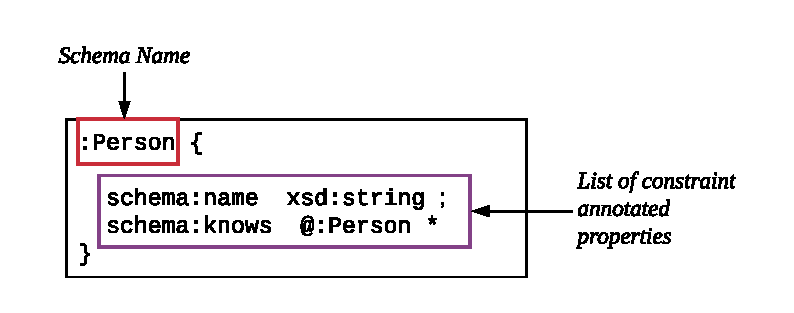
\includegraphics[scale=0.7]{images/shex-example-parts.pdf}
    \centering
    \caption[Shape expression modeling the properties of a Person]{Shape expression modeling the properties of a Person.}
    \label{fig:prop-def-shape-diagram}
\end{figure}


% S E C T I O N   P L A I N   O B J E C T S   E X P R E S I V I T Y

\section{Plain Objects Expressivity}\label{sec:poe}
Plain objects can be coded in any object oriented programming language, or at least in
any language that supports this paradigm. First we will explore how plain objects are 
generally coded, then how the language increases or decreases the expressivity and
finally we will generalize the core concepts that can be expressed by any plain object
codification.

\begin{figure}
    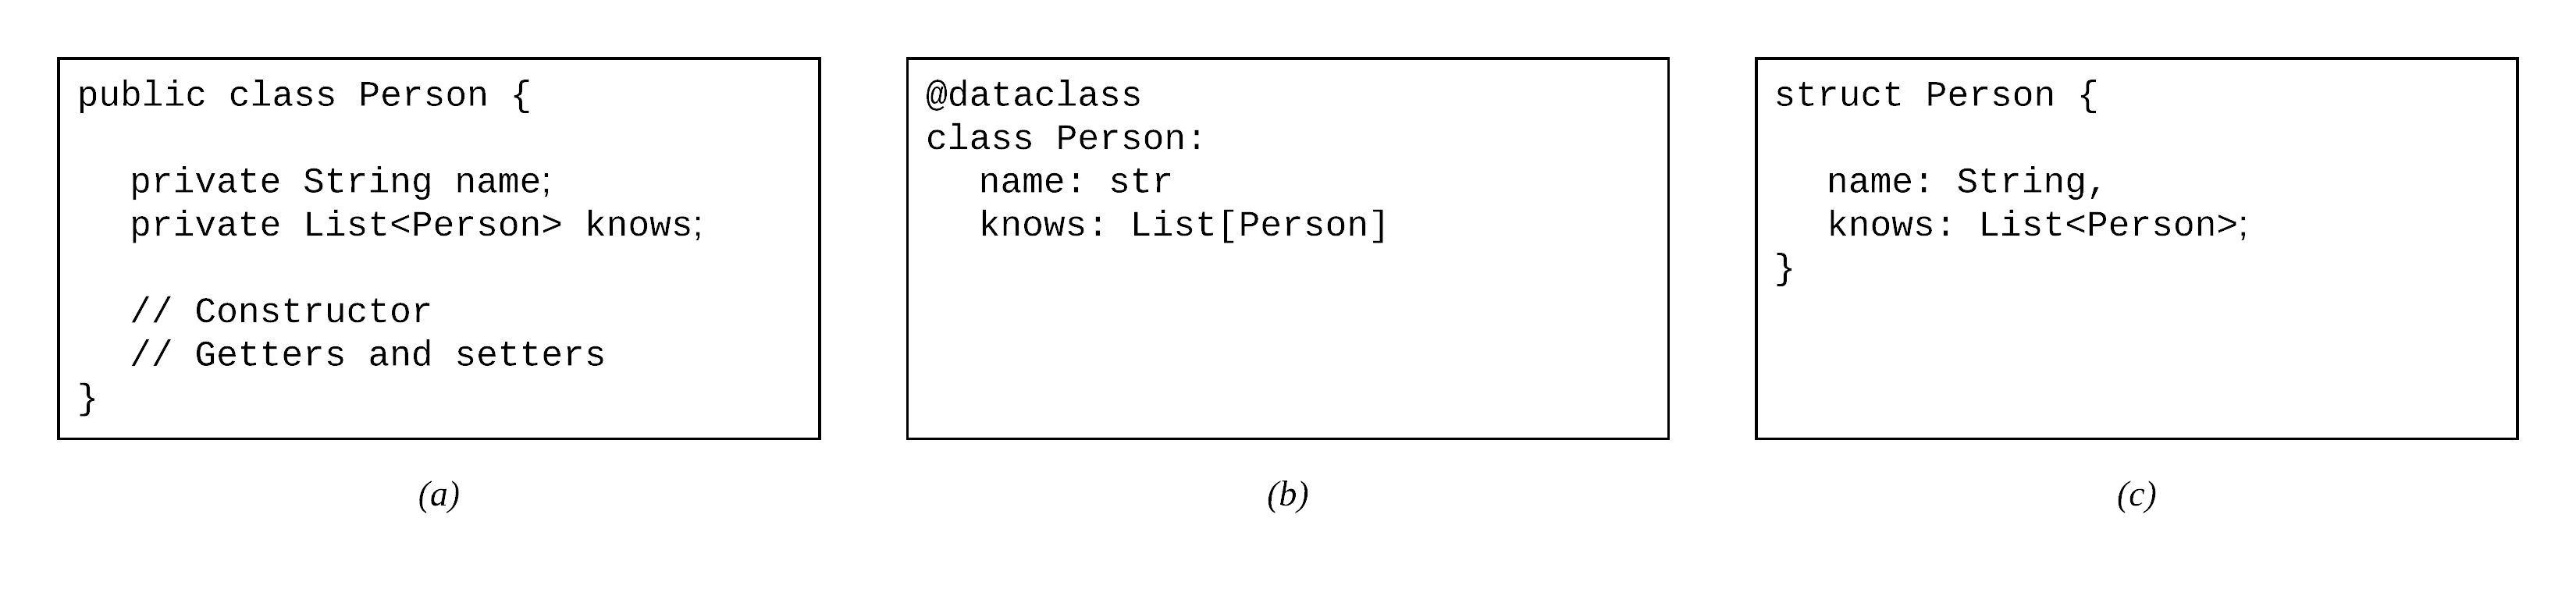
\includegraphics[width=\textwidth]{images/codings-exmaple.png}
    \centering
    \caption[Java, Python and Rust codings of Person object.]{Java, Python and Rust codings of Person object. 
    \textit{a} corresponds to Java, \textit{b} corresponds to Python and \textit{c} corresponds to Rust.}
    \label{fig:person-codings}
\end{figure}


\subsection{Plain Objects Structure}
From the existing programming languages we can infeer the general structure of plain objects. For this porpuse
we take the PYPL Index \textit{(PopularitY of Programming Language)} \footnote{\url{http://pypl.github.io/PYPL.html}}
from June 2020 and take the 2 most used programming languages that support the object oriented paradigm,
those would be Java and Python. And then, just to enlarge the scope we will take Rust because it is a new programming
language that includes lots of features.

\cref{fig:person-codings} shows three models that correspond to the codification of the Person schema from
\cref{fig:shex-translate-small}. For example if we analyze the Java fragment, that seems to be the most complex
one out of the three fragments we can see in \cref{fig:java-analysis} that it is composed by the \textit{Schema Name},
the \textit{List of Type Annotated Properties} and some \textit{Language Specific Code}. This corelates to the other
two programming languages as they also contain this three elements.

\begin{figure}
    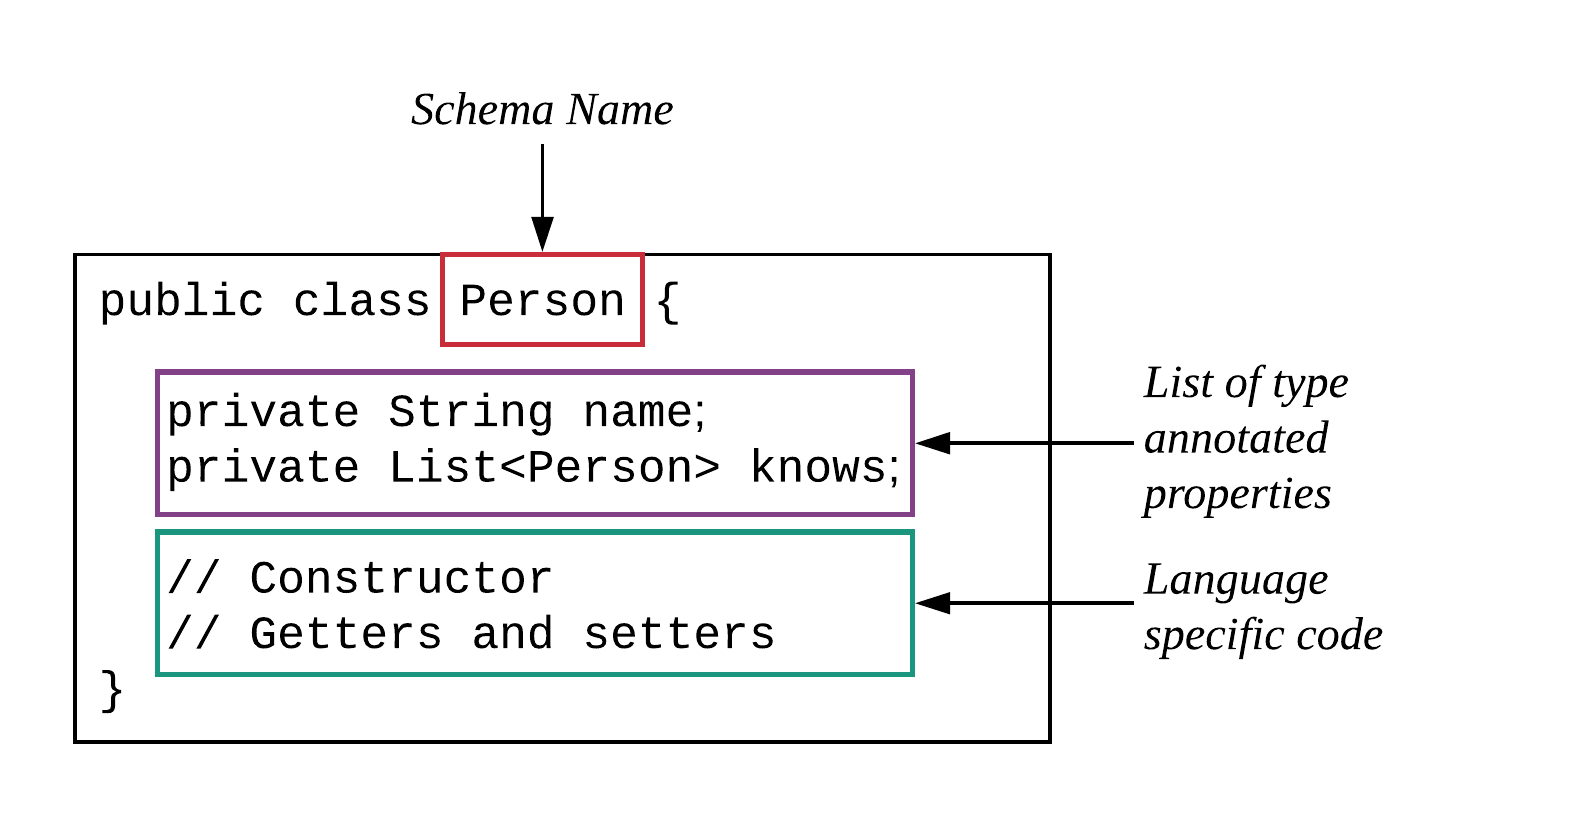
\includegraphics[scale=0.2]{images/java-analysis.png}
    \centering
    \caption[Java plain object decomposition.]{Java plain object decomposition.}
    \label{fig:java-analysis}
\end{figure}

It is important to note that although the composition of the property identifiers may
vary a little in each programming language, the type system is specific and sure to
change in each language. This is why we must explore to what extent it affects the
type system of each language. And if, therefore, it can be generalized.

\subsection{Plain Objects Formalization}
In order to compare the expressiveness of plain objects with other systems, we will carry out a
formalization based on their structure and content. Let $N$ be the set of all possible variable
identificators in a programing language and $T_{pl}$ the set of all possible types in a programming
language. Then a type annotated property is defined as
\begin{equation}\label{eq:plain-object}
(n,t_{pl}) \in N \times T_{pl},
\end{equation}
where $n$ is the identifier of the property and $t_{pl}$ the specific programing language type. That implies that a plain object
\begin{equation}
c \subseteq N \times T_{pl}.
\end{equation}
is a set of type annotated properties. Thus, an object domain model
\begin{equation}\label{eq:exp-m}
M = \{ c \mid c \subseteq N \times T_{pl} \}.
\end{equation}
is a set of plain objects. Therefore, $e(plain\ objects) = N \times T_{pl} $.

\subsection{Plain Objects Language Expressivity Dependence}
In \cref{fig:person-codings} we can see that all of three languages use similar types to represent the Person model. But with
just one example we cannot generalize that the language does not affect the expressivity of the plain objects. In order to
test that condition and prove that the language affects or does not affect the expressivity of plain objects we will need first
to find two \textit{type-independent languages}.

\begin{definition}[Type-independent languages]
    Two languages $L_1$ and $L_2$ are type-independent if and only if one of the languages contains a type that cannot be
    represented by means of a linear combination of any other type of the other language.
\end{definition}

For example, lets take Java \textit{$L_1$} and Rust \textit{$L_2$}, examples \textit{(a)} and \textit{(c)} from \cref{fig:person-codings}.
Rust contains the type $Either<A,B>$, this type allows the type $A$ or $B$ and when accessed is not an $Either$ is either $A$ or $B$. In
Java there is no $Either$ type, and someone can say that we could achieve a similar type by using inheritance and classes composition. But
at the end when accessed the type would be the type of the upper class. \textbf{Therefore Java and Rust are type-independent languages}.

Now in order to see if the expressivity depends on the types of a language let's assign values to Java and Rust by using the same
$Either<A,B>$ type. As can be see in \cref{fig:java-rust-comparison} Java does not allow to express the same as we are expressing in Rust
in this example. And therefore, we can conclude that the expressivity of plain object is strongly related to the build-in types that
the programming language in which they are coded provides.

\begin{center}
	\noindent\begin{minipage}[t]{.4\textwidth}
        \begin{lstlisting}[language=Java,frame=topline,numbers=left,title=\scriptsize{Person Rust Struct},
            basicstyle=\ttfamily\scriptsize]{a}
struct Person {
    name: String,
    knows: List<Person>,
    owningPet: Either<Dog,Cat>,
}
		\end{lstlisting}
	\end{minipage}\hfill
	\begin{minipage}[t]{.5\textwidth}
        \begin{lstlisting}[language=Java, frame=t,numbers=left,title=\scriptsize{Person Java Object},
            basicstyle=\ttfamily\scriptsize]{b}
// Imports...
public class Person {
    private String name;
    private List<Person> knows;
    private Pet owningPet;
    // Constructor...
    // Getters and Setters...
}
		\end{lstlisting}
	\end{minipage}
    \captionof{figure}{Rust struct modeling a \texttt{Person} to the left.
    And the most similar approximation in Java to te right. In the Java approximation the Pet class is an interface
    that it is inherited by the Cat and Dog classes, that way we allow to store in the variable \texttt{owningPet}
    values of type Cat and Dog.}
	\label{fig:java-rust-comparison}
\end{center}


\subsection{Plain Objects Expressivity Generalization}
In order to obtain a generalization of the plain objects represented by means of object-oriented programming languages,
we will base ourselves on \cref{eq:plain-object} where we defined the composition of a plain object, in this way the
generalization would be as indicated in \cref{fig:po-generalization}. As can be seen this generalization is not complete
as it does not include the production for the \texttt{type}. This is because we have not generalized the type system of the
object oriented programming languages yet.

\begin{figure}
    \begin{lstlisting}[numbers=left,basicstyle=\ttfamily\small]
    plain object     ::= (ID type)+
    \end{lstlisting}
    \caption[Plain Objects Partial Generalization]{Plain Objects Partial Generalization.}
    \label{fig:po-generalization}
\end{figure}

However, and motivated by not to over-extend the scope of this work, instead of extracting a generalization for all the possible types
that can be used in each object-oriented programming language, we will try to create this abstraction projecting the
most common types used by XML Schema (xsd) \cite{xmlschemasimpleelements}. The main reason, is that in RDF, and therefore in ShEx, xsd is the most widely
used type system and the standard of w3c. This leads us to the generalization from \cref{fig:po-generalization-complete} where we re-use the
\texttt{xsd} types and add the \texttt{ID} that actually represents compound types, that is types that are in fact plain objects.

\begin{figure}
    \begin{lstlisting}[numbers=left,basicstyle=\ttfamily\small]
    plain object     ::= (ID type)+
    type             ::= REAL | LIST[type] | STRING | BOOLEAN | ID
    \end{lstlisting}
    \caption[Plain Objects Complete Generalization]{Plain Objects Complete Generalization.}
    \label{fig:po-generalization-complete}
\end{figure}

% S E C T I O N   C O M P A R I S O N 

\section{Shape Expressions and Plain Objects Expressivity Comparison}

Previous section cover the expressivity of Shape Expressions and Plain Objects.
In this section we compare both expressivities and expose if both expressivities
are compatible or not. \cref{eq:exp-shape} showed that the expressiveness of the
schemes depends on $P \times T_{rdf} \times C$. Meanwhile \cref{eq:exp-m} showed
that the expressivity of object domain models depends on $P \times T_{pl}$. In
\cref{sec:poe} we restrict the types that a plain object property might have.
Let $T_g$ be the set of all allowed types in a plain object $\{ Real, List_{T_g}, String, Boolean, Reference \}$.
Then, $e(plain\ objects) = N \times T_g$. We will compare now if $P \times T_{rdf} \times C = N \times T_g$.
For that purpose we will compare each space separately to see if they represent the same.

\begin{equation}\label{eq:restrict-spaces}
    \left.\begin{matrix}
        P \rightarrow\ All\ the\ URIs.
     \\ N \rightarrow\ All\ the\ identifiers.
     \end{matrix}\right\} N \subseteq P\\
     \left.\begin{matrix}
        T_{rdf} \rightarrow\ All\ RDF\ types.
     \\ T_{g} \rightarrow\ All\ allowed\ plain\ objects\ types.
     \end{matrix}\right\} T_g \subseteq T_{rdf}\\
\end{equation}

\begin{figure}
    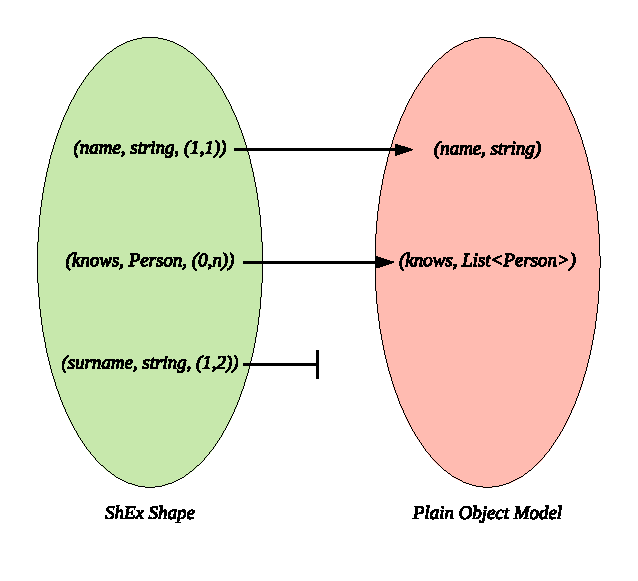
\includegraphics[scale=1]{images/shex-lite-mapping.pdf}
    \centering
    \caption[Mapping function from ShEx to Plain Object]{Mapping function from ShEx to Plain Object.}
    \label{fig:mapping-f}
\end{figure}

Here we can see that the $C$ has no space to compare with as $s$ does not include any information about this.
In $s$ instead of using a cardinality there is a list type that represents the cardinality $(0, \infty)$.

From here we see that $e(shex\ micro\ syntax) \not\leq e(plain\ objects)$. So that answers the question.
As the expressivity of Shape Expressions Micro Compact Syntax is greater than the expressivity of the
defined Object Domain Models we cannot transform all the existing schemas from $S$ to plain objects from $M$.
That can be easily proven also by assigning values to S and trying to map them in to $M$. \cref{eq:values-mapping}
and \cref{fig:mapping-f} illustrate this.

\begin{equation}\label{eq:values-mapping}
    \begin{aligned}
(name,string,(1,1)) & \rightarrow & (name,string)\\
(knows,Person,(0,\infty)) & \rightarrow & (knows,List[Person])\\
(surname,string,(1,2)) & \rightarrow & \times \\
(enrolled,Person,(2,\infty)) & \rightarrow & \times \\
(length,inches,(1,1)) & \rightarrow & \times  
    \end{aligned}
\end{equation}

\cref{fig:mapping-f} also illustrates perfectly that there exists some cases where the trasnformation can take
place. Now we will focus on finding those cases. From \cref{eq:restrict-spaces} we know that both $N \subseteq P$
and $T_g \subseteq T_{rdf}$ and previously we saw that if $c \in {(1,1), (0,\infty)}$ we can represent that by means
of the type List. Therefore
\begin{equation}\label{eq:restriction}
    \forall\ (p,t,c) \in N \times T_g \times \{(1,1),(0,\infty)\}   
\end{equation}

both systems share the same expressivity. Which implies that a shape' $s' \subseteq N \times T_g \times \{(1,1),(0,\infty)\}$
is a set of triple constraints that can be represented as type annotated properties. And therefore
$S'=\{s \mid s' \subseteq N \times T_g \times \{(1,1),(0,\infty)\} \}$ is equivalent to $M = \{ c \mid c \subseteq N \times T_{g} \}$.